\documentclass[11pt,a4paper]{article}

% ============================================================================
% Style: matched to the RASD (Mohammadi Masoudi Ramin, Rev. 0.5, May 2026)
% ============================================================================
\usepackage[T1]{fontenc}
\usepackage[utf8]{inputenc}
\usepackage[margin=2.5cm]{geometry}
\usepackage{hyperref}
\usepackage{booktabs}
\usepackage{longtable}
\usepackage{array}
\usepackage{xcolor}
\usepackage{colortbl}
\usepackage{listings}
\usepackage{tikz}
\usepackage{amsmath}
\usepackage{amssymb}
\usepackage{graphicx}
\usepackage{fancyhdr}
\usepackage{titlesec}
\usepackage{enumitem}
\usepackage{float}
\usepackage{multirow}
\usepackage{tabularx}
\usepackage{tcolorbox}
% Compact ToC spacing — the default leaves too much vertical air,
% pushing entries past §9 onto a second page. titletoc lets us shrink
% the spacing around each section entry so the full ToC fits on one page.
\usepackage{titletoc}
\titlecontents{section}[1.5em]
  {\vspace{1pt}\small}
  {\contentslabel{1.5em}}
  {}
  {\titlerule*[0.5pc]{.}\contentspage}
\titlecontents{subsection}[3.8em]
  {\vspace{-1pt}\footnotesize}
  {\contentslabel{2.3em}}
  {}
  {\titlerule*[0.5pc]{.}\contentspage}
\titlecontents{subsubsection}[6em]
  {\vspace{-1pt}\footnotesize}
  {\contentslabel{2.6em}}
  {}
  {\titlerule*[0.5pc]{.}\contentspage}

\usetikzlibrary{shapes,arrows,positioning,fit,calc,backgrounds,decorations.pathreplacing,matrix,shapes.geometric,arrows.meta}
\tcbuselibrary{skins,breakable}

% ---- Colours: identical to the RASD --------------------------------------
\definecolor{docblue}{RGB}{0,51,102}
\definecolor{doclblue}{RGB}{0,85,128}
\definecolor{reqbg}{RGB}{235,244,255}
\definecolor{reqframe}{RGB}{70,100,150}
\definecolor{nfrbg}{RGB}{240,255,240}
\definecolor{nfrframe}{RGB}{40,120,70}
\definecolor{codebg}{RGB}{247,247,247}
\definecolor{tabhead}{RGB}{0,51,102}
\definecolor{rowalt}{RGB}{243,247,255}
\definecolor{warnbg}{RGB}{255,251,230}
\definecolor{warnframe}{RGB}{170,120,0}
\definecolor{stateblue}{RGB}{0,70,140}
\definecolor{statefill}{RGB}{220,232,250}
\definecolor{ddbg}{RGB}{248,243,230}
\definecolor{ddframe}{RGB}{160,120,40}

\hypersetup{
  colorlinks=true, linkcolor=docblue, urlcolor=doclblue, citecolor=docblue,
  pdftitle={NEORV32 Ascon-AEAD128 Hardware Accelerator: Development Report},
  pdfauthor={Mohammadi Masoudi Ramin}
}

\titleformat{\section}
  {\Large\bfseries\color{docblue}}{\thesection}{1em}{}
  [\color{docblue}\rule{\linewidth}{0.6pt}]
\titleformat{\subsection}
  {\large\bfseries\color{docblue}}{\thesubsection}{1em}{}
\titleformat{\subsubsection}
  {\normalsize\bfseries\color{doclblue}}{\thesubsubsection}{1em}{}

\pagestyle{fancy}\fancyhf{}
\fancyhead[L]{\small\color{docblue}\textbf{NEORV32 Ascon-AEAD128 Hardware Accelerator}}
\fancyhead[R]{\small\color{docblue}Development Report}
\fancyfoot[C]{\small\thepage}
\renewcommand{\headrulewidth}{0.4pt}

\lstdefinelanguage{myc}{
  morekeywords={int,uint8_t,uint32_t,void,const,return,if,while,static,inline,for,bool,true,false,struct},
  morecomment=[l]{//}, morecomment=[s]{/*}{*/},
  morestring=[b]"
}
\lstdefinelanguage{shell}{
  basicstyle=\ttfamily\footnotesize,
}
\lstset{
  backgroundcolor=\color{codebg},
  basicstyle=\ttfamily\footnotesize,
  breaklines=true, frame=single, rulecolor=\color{gray!35},
  numbers=none,
  keywordstyle=\color{docblue}\bfseries,
  commentstyle=\color{gray!65}\itshape,
  stringstyle=\color{doclblue},
  xleftmargin=2em, framexleftmargin=2em,
  aboveskip=8pt, belowskip=6pt,
  columns=fullflexible
}

% ---- Macros: requirement / NFR / decision / warn boxes -------------------
\newcommand{\req}[3]{%
  \begin{tcolorbox}[
    enhanced, colback=reqbg, colframe=reqframe,
    arc=2pt, boxrule=0.5pt,
    left=6pt, right=6pt, top=3pt, bottom=3pt,
    attach boxed title to top left={yshift=-2mm, xshift=8pt},
    boxed title style={colback=reqframe, arc=2pt, boxrule=0pt,
                       left=4pt, right=4pt, top=2pt, bottom=2pt},
    title={\small\bfseries\color{white}#1\enspace\textbar\enspace\textit{#2}},
    before upper={\small}
  ]
  #3
  \end{tcolorbox}\vspace{3pt}}

\newcommand{\nfr}[3]{%
  \begin{tcolorbox}[
    enhanced, colback=nfrbg, colframe=nfrframe,
    arc=2pt, boxrule=0.5pt,
    left=6pt, right=6pt, top=3pt, bottom=3pt,
    attach boxed title to top left={yshift=-2mm, xshift=8pt},
    boxed title style={colback=nfrframe, arc=2pt, boxrule=0pt,
                       left=4pt, right=4pt, top=2pt, bottom=2pt},
    title={\small\bfseries\color{white}#1\enspace\textbar\enspace\textit{#2}},
    before upper={\small}
  ]
  #3
  \end{tcolorbox}\vspace{3pt}}

\newcommand{\dd}[3]{%
  \begin{tcolorbox}[
    enhanced, colback=ddbg, colframe=ddframe,
    arc=2pt, boxrule=0.5pt,
    left=6pt, right=6pt, top=3pt, bottom=3pt,
    attach boxed title to top left={yshift=-2mm, xshift=8pt},
    boxed title style={colback=ddframe, arc=2pt, boxrule=0pt,
                       left=4pt, right=4pt, top=2pt, bottom=2pt},
    title={\small\bfseries\color{white}#1\enspace\textbar\enspace\textit{#2}},
    before upper={\small}
  ]
  #3
  \end{tcolorbox}\vspace{3pt}}

\newcommand{\warn}[1]{%
  \begin{tcolorbox}[
    enhanced, colback=warnbg, colframe=warnframe,
    arc=2pt, boxrule=0.5pt, left=6pt, right=6pt, top=3pt, bottom=3pt,
    before upper={\small}
  ]
  \textbf{\color{warnframe}Important:} #1
  \end{tcolorbox}\vspace{3pt}}

% Table style
\renewcommand{\arraystretch}{1.18}
\arrayrulecolor{black!35}

% ============================================================================
\begin{document}

\begin{titlepage}
\centering
\vspace*{2cm}
{\color{docblue}\rule{\linewidth}{1.2pt}}
\vspace{0.4cm}\par
{\Huge\bfseries\color{docblue}NEORV32 Accelerator for Cryptography\par}
\vspace{0.4cm}
{\Large\color{doclblue}Ascon-AEAD128 Hardware Accelerator\par}
{\Large\color{doclblue}\textit{Development Report}\par}
\vspace{0.2cm}
{\color{docblue}\rule{\linewidth}{1.2pt}}
\vspace{2.2cm}\par

\begin{tabularx}{0.85\linewidth}{>{\bfseries\color{docblue}}lX}
Author             & Mohammadi Masoudi Ramin\\[2pt]
Project Title      & NEORV32 Accelerator for Cryptography\\[2pt]
Companion          & RASD, Rev.~0.5 (May~15,~2026)\\[2pt]
Target Platform    & NEORV32 RISC-V SoC, Sipeed Tang Nano 9K\\[2pt]
FPGA Device        & Gowin GW1NR-9 (8640 LUT4, 6480 FF, 26 BSRAM)\\[2pt]
Integration        & NEORV32 Custom Functions Subsystem (CFS)\\[2pt]
Algorithm          & Ascon-AEAD128, NIST SP~800-232 (Aug.~2025)\\[2pt]
HDL                & Verilog accelerator; VHDL CFS wrapper\\[2pt]
Document Rev.      & 1.0\\[2pt]
Date               & \today\\
\end{tabularx}

\vfill
\begin{tcolorbox}[colback=reqbg, colframe=reqframe, arc=2pt, width=0.9\linewidth]
\small
This document is the development companion to the Requirements \& Design
Document (RASD). It records every implementation decision, the four-layer
verification strategy and its concrete evidence, the synthesis and
silicon-validation results, the configurable architecture-exploration
framework, and a side-by-side comparison with the official Ascon
hardware reference (Primas et al., IAIK Graz). The RASD specifies what
the system shall do; this document records what was built, what was
learned, and what was deliberately chosen along the way.
\end{tcolorbox}
\vspace{1.2cm}
\end{titlepage}

\tableofcontents
\thispagestyle{fancy}
\newpage

% ============================================================================
\section{Introduction}

\subsection{Purpose}
This document records the development of an Ascon-AEAD128 hardware
accelerator integrated as a Custom Functions Subsystem (CFS) on the
NEORV32 RISC-V soft-core, together with the broader
architecture-exploration framework that grew up around the
single-instance accelerator. It is the technical record that the
RASD~§10.7 reserved to a ``separate development report''.

\subsection{Relationship to the RASD}

\begin{center}
\begin{tabular}{p{0.46\linewidth}p{0.46\linewidth}}
\toprule
\rowcolor{tabhead!20}\textbf{RASD (Rev.~0.5)} & \textbf{Development Report (this document)}\\
\midrule
Defines the algorithm, the register map, the FSM, and the functional and non-functional requirements that the implementation \emph{shall} satisfy. &
Records what was actually built, the design decisions that were taken, the verification evidence collected, the synthesis numbers measured, the architecture-exploration framework, and the comparison against the official ascon-hardware reference.\\
\midrule
Scope: Ascon-AEAD128 on NEORV32 + Tang Nano 9K. &
Scope: everything in the RASD plus the broader \emph{generator} that was developed during the work --- five backend variants, an AXI-stream data plane, an AXI-MMIO bridge, the configuration vocabulary in \texttt{ascon\_arch/}, and the multi-layer verification flow that includes a Verilator co-simulation of the integrated SoC.\\
\midrule
References future development. &
Lists every design decision (\textsection\ref{sec:dd}), maps every RASD requirement to its implementation (\textsection\ref{sec:rasd-map}), and shows what was verified and where (\textsection\ref{sec:ver}).\\
\bottomrule
\end{tabular}
\end{center}

\subsection{Document Conventions}

\begin{center}
\begin{tabular}{p{0.3\linewidth}p{0.62\linewidth}}
\toprule
\rowcolor{tabhead!20}\textbf{Box type} & \textbf{Meaning}\\
\midrule
\colorbox{reqbg}{\strut\quad\textbf{FR-xxx}\quad}     & RASD functional requirement (referenced; the full text is in the RASD).\\
\colorbox{nfrbg}{\strut\quad\textbf{NFR-xxx}\quad}    & RASD non-functional requirement (referenced).\\
\colorbox{ddbg}{\strut\quad\textbf{DD-xxx}\quad}      & A design decision made during development. Each lists rationale, alternatives considered, consequences, and where it is implemented.\\
\colorbox{warnbg}{\strut\quad\textbf{Important}\quad} & A pitfall or non-obvious constraint future readers should know about.\\
\bottomrule
\end{tabular}
\end{center}

% ============================================================================
\section{System Overview}

\subsection{High-Level Architecture}

Figure~\ref{fig:arch} shows the system organised as five horizontal
layers, each implemented in a separate part of the repository. The
arrows are control/data flow; the dashed boundary marks what is
on-chip versus off-chip.

\begin{figure}[H]
\centering
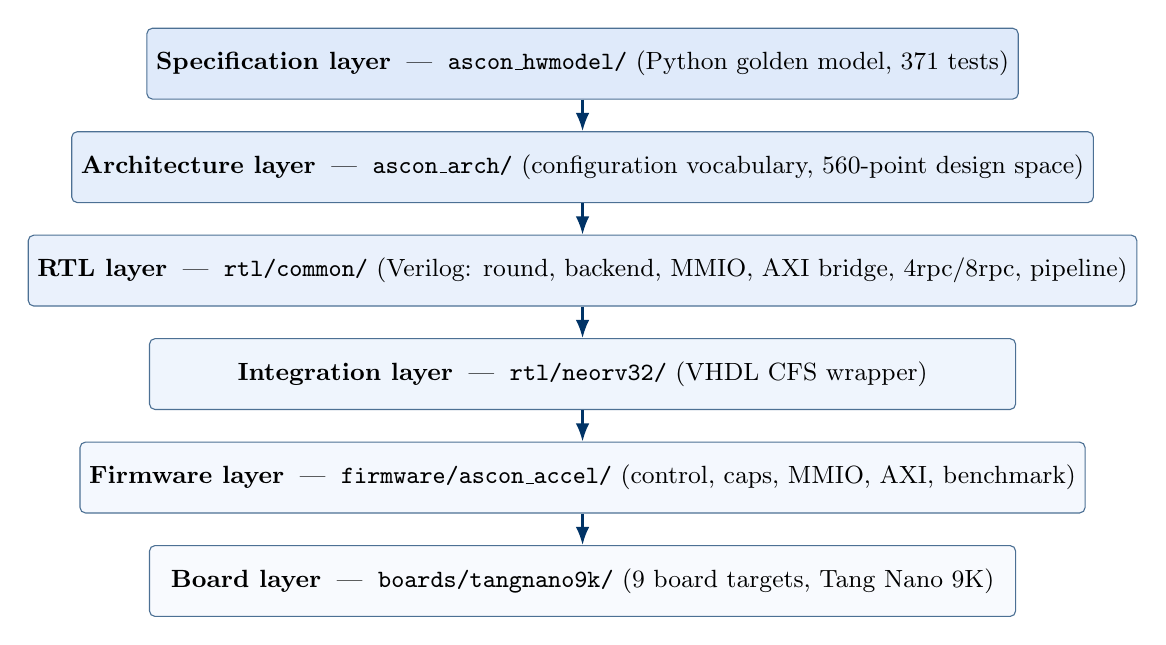
\begin{tikzpicture}[
  font=\small,
  layer/.style={rectangle, draw=docblue!70, fill=statefill, minimum width=11cm, minimum height=0.9cm, rounded corners=2pt, align=center},
  edge/.style={->, >=Latex, thick, draw=docblue},
  node distance=0.4cm
]
\node[layer, fill=statefill!90] (l1) {\textbf{Specification layer} \;---\; \texttt{ascon\_hwmodel/} (Python golden model, 371 tests)};
\node[layer, fill=statefill!75, below=of l1] (l2) {\textbf{Architecture layer} \;---\; \texttt{ascon\_arch/} (configuration vocabulary, 560-point design space)};
\node[layer, fill=statefill!60, below=of l2] (l3) {\textbf{RTL layer} \;---\; \texttt{rtl/common/} (Verilog: round, backend, MMIO, AXI bridge, 4rpc/8rpc, pipeline)};
\node[layer, fill=statefill!45, below=of l3] (l4) {\textbf{Integration layer} \;---\; \texttt{rtl/neorv32/} (VHDL CFS wrapper)};
\node[layer, fill=statefill!30, below=of l4] (l5) {\textbf{Firmware layer} \;---\; \texttt{firmware/ascon\_accel/} (control, caps, MMIO, AXI, benchmark)};
\node[layer, fill=statefill!20, below=of l5] (l6) {\textbf{Board layer} \;---\; \texttt{boards/tangnano9k/} (9 board targets, Tang Nano 9K)};
\draw[edge] (l1) -- (l2);
\draw[edge] (l2) -- (l3);
\draw[edge] (l3) -- (l4);
\draw[edge] (l4) -- (l5);
\draw[edge] (l5) -- (l6);
\end{tikzpicture}
\caption{Repository layering. Each layer corresponds to a directory; each
arrow corresponds to an actual code-level dependency (e.g.\ \texttt{rtl/}
sources are included by the board top files, the VHDL wrapper instantiates
the Verilog backend, the firmware drives the registers defined in
\texttt{rtl/common/ascon\_accel\_regs.vh}).}
\label{fig:arch}
\end{figure}

\subsection{Integrated System Block Diagram}

\begin{figure}[H]
\centering
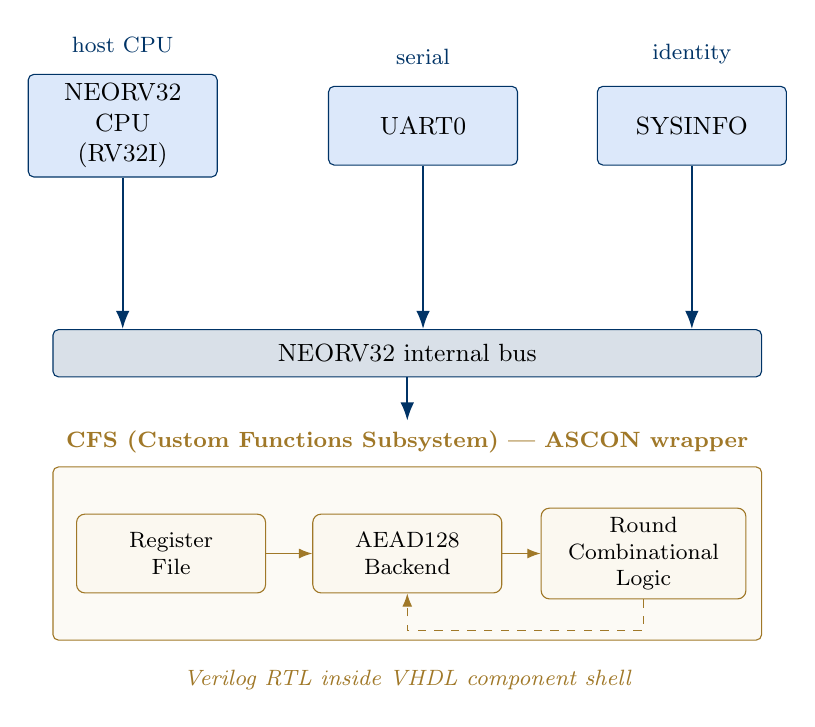
\begin{tikzpicture}[
  font=\small,
  blk/.style={rectangle, draw=docblue, fill=statefill, rounded corners=2pt, minimum width=2.4cm, minimum height=1cm, align=center},
  reg/.style={rectangle, draw=ddframe, fill=ddbg!60, rounded corners=3pt, minimum width=2.4cm, minimum height=1.0cm, align=center, font=\footnotesize},
  bus/.style={->, >=Latex, thick, draw=docblue},
  node distance=0.4cm
]
% Top row: CPU peripherals
\node[blk] (cpu) {NEORV32\\CPU\\(RV32I)};
\node[blk, right=1.4cm of cpu] (uart) {UART0};
\node[blk, right=1.0cm of uart] (sysinfo) {SYSINFO};

% Internal bus
\node[blk, below=1.0cm of cpu, minimum width=9.0cm, minimum height=0.6cm, fill=docblue!15]
  (bus) at ($(cpu.south)!0.5!(sysinfo.south) + (0,-1.0)$) {NEORV32 internal bus};

% CFS title goes ABOVE the box so it never overlaps the border.
\node[font=\footnotesize\bfseries, color=ddframe, below=0.55cm of bus]
  (cfs_title) {CFS (Custom Functions Subsystem) --- ASCON wrapper};

% CFS box: sized to contain the three reg nodes
\node[draw=ddframe, fill=ddbg!40, rounded corners=2pt, minimum width=9.0cm, minimum height=2.2cm,
      below=0.05cm of cfs_title.south, anchor=north]
  (cfs) {};

% Three internal blocks, evenly spaced within the CFS box
\node[reg] at ($(cfs.center)+(-3.0,0)$) (regs) {Register\\File};
\node[reg] at ($(cfs.center)+(0.0,0)$)  (backend) {AEAD128\\Backend};
\node[reg, minimum width=2.6cm] at ($(cfs.center)+(3.0,0)$) (round) {Round\\Combinational\\Logic};

\draw[->, >=Latex, draw=ddframe] (regs) -- (backend);
\draw[->, >=Latex, draw=ddframe] (backend) -- (round);
% Feedback arc: registered-state loop
\draw[->, >=Latex, draw=ddframe, dashed] (round.south) -- ++(0,-0.4) -| (backend.south);

% Bus connections (CPU -> bus, bus -> CFS)
\draw[bus] (cpu) -- (cpu |- bus.north);
\draw[bus] (uart) -- (uart |- bus.north);
\draw[bus] (sysinfo) -- (sysinfo |- bus.north);
\draw[bus] (bus.south) -- (cfs_title);

% Labels above the top row
\node[font=\footnotesize, color=docblue, above=0.15cm of cpu] {host CPU};
\node[font=\footnotesize, color=docblue, above=0.15cm of uart] {serial};
\node[font=\footnotesize, color=docblue, above=0.15cm of sysinfo] {identity};

% Footer: implementation note BELOW the CFS box, not inside
\node[font=\footnotesize\itshape, color=ddframe, below=0.25cm of cfs.south]
  {Verilog RTL inside VHDL component shell};
\end{tikzpicture}
\caption{Integrated NEORV32 + ASCON-CFS system. The CFS shell is VHDL;
its body wraps the project's Verilog backend, register file, and
combinational round logic. The dashed arc is the per-cycle permutation
feedback inside the backend.}
\label{fig:soc}
\end{figure}

\subsection{Verification Pyramid}

\begin{figure}[H]
\centering
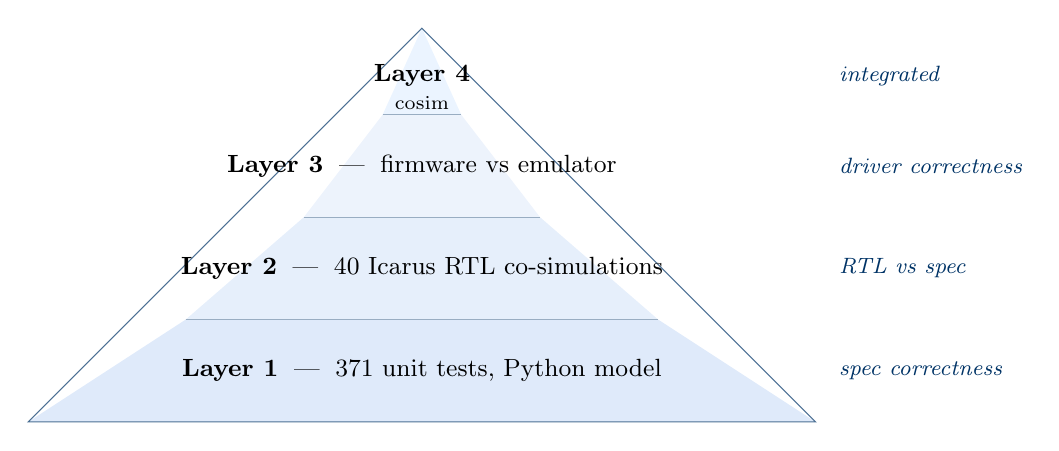
\begin{tikzpicture}[font=\small]
\fill[statefill!90] (0,0) -- (10,0) -- (8,1.3) -- (2,1.3) -- cycle;
\fill[statefill!70] (2,1.3) -- (8,1.3) -- (6.5,2.6) -- (3.5,2.6) -- cycle;
\fill[statefill!50] (3.5,2.6) -- (6.5,2.6) -- (5.5,3.9) -- (4.5,3.9) -- cycle;
\fill[reqbg]        (4.5,3.9) -- (5.5,3.9) -- (5,5) -- cycle;
\draw[draw=docblue!70] (0,0) -- (10,0) -- (5,5) -- cycle;
\draw[draw=docblue!40] (2,1.3) -- (8,1.3);
\draw[draw=docblue!40] (3.5,2.6) -- (6.5,2.6);
\draw[draw=docblue!40] (4.5,3.9) -- (5.5,3.9);
\node at (5,0.65) {\textbf{Layer 1} \;---\; 371 unit tests, Python model};
\node at (5,1.95) {\textbf{Layer 2} \;---\; 40 Icarus RTL co-simulations};
\node at (5,3.25) {\textbf{Layer 3} \;---\; firmware vs emulator};
\node at (5,4.4) {\textbf{Layer 4}};
\node at (5,4.05) {\scriptsize cosim};
\node[right=5pt, font=\footnotesize\itshape, color=docblue] at (10,0.65)  {spec correctness};
\node[right=5pt, font=\footnotesize\itshape, color=docblue] at (10,1.95) {RTL vs spec};
\node[right=5pt, font=\footnotesize\itshape, color=docblue] at (10,3.25) {driver correctness};
\node[right=5pt, font=\footnotesize\itshape, color=docblue] at (10,4.4) {integrated};
\end{tikzpicture}
\caption{Verification pyramid. Each layer catches a different class of bug
and runs on open-source tooling only. Layer~4 (the Verilator co-simulation)
was added during development when on-silicon integration was found
infeasible on the GW1NR-9 with the open-source PnR flow.}
\label{fig:pyramid}
\end{figure}

% ============================================================================
\section{Design Decisions}
\label{sec:dd}

This section enumerates every substantive design decision made during
the project. Decisions are recorded as DD-xxx items with a fixed
rationale/alternatives/consequence structure so the reasoning behind
the implementation is auditable.

\subsection{Foundational Decisions}

\dd{DD-001}{Stable layered architecture}{
\textbf{Decision.} Separate the project into six layers: specification
(Python), architecture (Python configuration vocabulary), RTL, RTL
integration (VHDL CFS wrapper), firmware (C), and per-board bring-up.

\textbf{Rationale.} The accelerator and its surrounding software each
evolve at different rates and need different verification tooling.
Layering keeps each piece individually testable.

\textbf{Alternatives.} A single monolithic Verilog + C project, as in
most academic accelerator papers; rejected because it cannot support
multiple backends behind one firmware.

\textbf{Consequence.} Layer boundaries are enforced: no NEORV32 signals
in the Verilog backend (RASD NFR-006), no Verilog in the firmware. Allows
the same firmware binary to be re-used across all five FPGA backend
variants.

\textbf{Implemented in.} The entire repository layout (Fig.~\ref{fig:arch}).
}

\dd{DD-002}{Frozen firmware ABI}{
\textbf{Decision.} The firmware-facing register map and bus protocol
are treated as immutable. Hardware may change internally; the software
contract may not.

\textbf{Rationale.} Without this, every change to the backend would
ripple into the firmware; cosim correctness would not generalise to
other backends.

\textbf{Alternatives.} Versioned ABI with negotiation at boot; rejected
as overkill at this stage but kept reachable through the
\texttt{ABI\_VERSION} register (\texttt{0x00000001} today).

\textbf{Consequence.} The cosim result in §\ref{sec:cosim} applies to
all five backend variants without re-verification of the firmware.

\textbf{Implemented in.} \texttt{rtl/common/ascon\_accel\_regs.vh},
\texttt{firmware/ascon\_accel/ascon\_accel\_regs.h}.
}

\dd{DD-003}{Control plane vs.\ data plane split}{
\textbf{Decision.} Always present a CSR/MMIO control plane (mode, key,
nonce, lengths, start, status, tag, cycle counter, error code, capability
register). The \emph{data plane} (how AD/PT/CT bytes get to and from the
accelerator) is pluggable: word-based MMIO, AXI-stream, or a future
DMA path.

\textbf{Rationale.} The control plane is small, fixed, and naturally a
register file; it is the same on every CPU. The data plane has very
different needs depending on whether the accelerator sits next to a
single-issue CPU (cheap MMIO is fine), behind an AXI bus (streams are
better), or behind a DMA engine. Coupling them would force trade-offs
on both.

\textbf{Alternatives.} Single fused interface (RFC-style FIFO); rejected
because it makes capability discovery awkward.

\textbf{Consequence.} The capability register (offset \texttt{0x0C} in the
project's MMIO map) reports which data plane is present, so the C driver
can dispatch to the right transport.

\textbf{Implemented in.} \texttt{ascon\_accel\_mmio\_regs.v},
\texttt{ascon\_accel\_caps.c},
\texttt{ascon\_accel\_axis\_data.c} vs \texttt{ascon\_accel\_mmio\_data.c}.
}

\dd{DD-004}{Open-source-only toolchain}{
\textbf{Decision.} The whole flow (simulation, synthesis, place \& route,
bitstream pack, programming) is reproducible from \texttt{flake.nix}
using only open-source tools. No vendor EDA is required to build,
verify, or flash a working bitstream.

\textbf{Rationale.} Reproducibility, portability, transparency, and
the ability to invite future contributors without licence friction.

\textbf{Alternatives.} Gowin EDA, which would close the integrated
bitstream's place-and-route at $92.6\%$ LUT4. Rejected as the default
for the repository, but documented as a fall-back deployment route.

\textbf{Consequence.} Hits a hard placement-density wall at $\sim 92\%$
LUT4 on the GW1NR-9 (see §\ref{sec:silicon}). This is the dominant
non-functional constraint of the project.
}

\dd{DD-005}{FPGA: maximum throughput first}{
\textbf{Decision.} For FPGA targets, optimise primarily for throughput,
not area. Multiple rounds per clock cycle, $128$-bit AXI-stream data
plane, and fully pipelined permutations are first-class options. The
small GW1NR-9 is treated as a bring-up vehicle, not the eventual target.

\textbf{Rationale.} The benchmark target in RASD~§8.4 is a $\geq 2\times$
software-to-hardware speed-up; aggressive parallelism is the natural
lever to overshoot it.

\textbf{Consequence.} Five FPGA backend variants are realised (one,
four, eight rounds/cycle; MMIO and AXI-stream; fully pipelined
permutation primitive).
}

\dd{DD-006}{ASIC: area first}{
\textbf{Decision.} For ASIC targets, optimise primarily for area:
serial datapaths, $5$-bit-S-box-serial designs, hardcoded FSMs.

\textbf{Rationale.} ASIC NRE makes area-per-tape-out the dominant
cost; throughput requirements are typically modest in the
target use cases.

\textbf{Consequence.} ASIC datapaths are not yet implemented; the axis
exists in the configuration vocabulary and is reserved for future work.
}

\subsection{RTL Decisions}

\dd{DD-007}{Verilog (not VHDL) for the accelerator}{
\textbf{Decision.} Implement the accelerator in synthesisable Verilog;
keep VHDL strictly for the NEORV32 CFS wrapper.

\textbf{Rationale.} (i) Yosys + GHDL synth + Verilator handle mixed
HDLs cleanly only when each module is in one language; (ii) Verilog
is the most common HDL in lightweight-cryptography open-source
implementations.

\textbf{Trade-off.} The official Ascon hardware reference (Primas et
al., IAIK) is VHDL; the AhmetMALAL ascon-vhdl repository is VHDL;
this project intentionally departs from that lineage.

\textbf{Implemented in.} \texttt{rtl/common/*.v}, \texttt{*.vh}.
}

\dd{DD-008}{Combinational round, registered state}{
\textbf{Decision.} \texttt{ascon\_round\_comb.v} is purely combinational
($p_C \!\circ\! p_S \!\circ\! p_L$); the FSM in
\texttt{ascon\_aead128\_mmio\_backend.v} registers the $320$-bit state
between rounds.

\textbf{Rationale.} Single source of truth for one round, easy to
re-use in multi-round-per-cycle variants by composing $k$ instances
combinatorially.

\textbf{Consequence.} The $4$rpc and $8$rpc backends are
implementation-by-instantiation: same round module, deeper combinational
chain.

\textbf{Implemented in.} \texttt{ascon\_round\_comb.v},
\texttt{ascon\_round4\_comb.v}, \texttt{ascon\_round8\_comb.v}.
}

\dd{DD-009}{Constant-time tag comparison}{
\textbf{Decision.} Tag comparison reduces all $128$ bits via an
\texttt{XOR}-tree to a single \texttt{tag\_ok} flag in one cycle, with
no early termination.

\textbf{Rationale.} A naïve byte-by-byte comparison leaks how many
bytes of a forged tag matched. A single-cycle reduction has no
data-dependent timing.

\textbf{Implemented in.} \texttt{ascon\_aead128\_mmio\_backend.v} (RASD FR-012).
}

\dd{DD-010}{Buffer plaintext until tag verifies}{
\textbf{Decision.} During decryption, recovered plaintext is buffered
inside the accelerator and is not exposed on the output bus until the
finalisation permutation produces \texttt{tag\_ok = 1}. If verification
fails the buffer is invalidated.

\textbf{Rationale.} An AEAD streaming interface that exposes plaintext
during the streaming phase before the tag is checked invites
firmware-side mistakes that leak unauthenticated plaintext. Buffering
inside the accelerator removes the possibility entirely.

\textbf{Cost.} $256$-bit additional register (the buffer is sized for
the longest payload the bounded backend accepts).

\textbf{Implemented in.} \texttt{ascon\_aead128\_mmio\_backend.v}
(RASD FR-015).
}

\dd{DD-011}{Little-endian bus byte convention}{
\textbf{Decision.} All bus values are little-endian within each $64$-bit
word: $\texttt{bus[7:0]}$ is byte~$0$. KEY0 holds bytes 0--3 in order.

\textbf{Rationale.} Matches RV32 native byte order and the C
\texttt{load32\_le}/\texttt{store32\_le} helpers. Single, uniform
convention across RTL, testbenches, firmware, and tool-generated
vectors.

\textbf{Risk.} A flipped endianness assumption anywhere is the most
common AEAD bug class: it produces wrong ciphertext with no other
diagnostic. RASD~§9.1 calls this out explicitly.

\textbf{Implemented in.} All Verilog data buses,
\texttt{ascon\_accel\_mmio\_regs.v}, the C driver, and the testbench
generators.
}

\subsection{Integration Decisions}

\dd{DD-012}{NEORV32 CFS as the host-attach point}{
\textbf{Decision.} Wrap the Verilog accelerator in a VHDL component
\texttt{neorv32\_cfs\_ascon} that drops into the standard NEORV32
\texttt{CFS} slot.

\textbf{Rationale.} NEORV32's CFS slot is exactly designed for this
class of integration: a $64$-byte MMIO window with bus, IRQ, and
optional clock/reset hand-shakes already wired up by the CPU. No
top-level NEORV32 surgery needed; the wrapper is a drop-in.

\textbf{Implemented in.} \texttt{rtl/neorv32/neorv32\_cfs\_ascon.vhd}
(RASD FR-014).
}

\dd{DD-013}{Two NEORV32 board tops: MMIO and AXI-stream}{
\textbf{Decision.} Provide two integrated SoC boards:
\texttt{neorv32\_mmio} (CFS + MMIO data plane) and
\texttt{neorv32\_stream\_axis\_mmio} (CFS + AXI-stream data plane via
an AXI-MMIO bridge).

\textbf{Rationale.} Lets a single firmware binary be retargeted from
``simple register file'' to ``streaming pipeline'' purely by changing
the board target. The capability register reports which one is present.

\textbf{Implemented in.}
\texttt{boards/tangnano9k/neorv32\_mmio/},
\texttt{boards/tangnano9k/neorv32\_stream\_axis\_mmio/}.
}

\dd{DD-014}{Standalone board targets for incremental bring-up}{
\textbf{Decision.} In addition to the integrated SoC, the repository
contains seven standalone Tang Nano 9K targets that isolate one part
of the system on real silicon (cf.\ Table~\ref{tab:targets}).

\textbf{Rationale.} Debugging the integrated bitstream on open-source
PnR is slow; debugging from LEDs is hard. Having a $16\%$-LUT
algorithmic-only target (\texttt{kat\_slow}) and a separate
$\sim 1700$-LUT MMIO-only target (\texttt{mmio\_slow}) lets a
ten-minute synth/flash cycle confirm each subsystem on real silicon
without going through the bigger build.

\textbf{Outcome.} Both \texttt{kat\_slow} and \texttt{mmio\_slow} are
silicon-verified PASS via on-board LEDs (§\ref{sec:silicon}).
}

\subsection{Firmware Decisions}

\dd{DD-015}{Firmware library, not monolithic binary}{
\textbf{Decision.} The driver is a static library (\texttt{ascon\_accel.c}
plus its transport, capability, and control modules) that the benchmark
firmware (\texttt{neorv32\_ascon\_benchmark/main.c}) links against.

\textbf{Rationale.} A separate library can be linked into any host
program --- including the host-side Python emulator used in
Layer~3 --- without source duplication. This is what makes Layer~3
verification (same C code, simulated transport) meaningful.

\textbf{Implemented in.} \texttt{firmware/ascon\_accel/*.c, *.h}.
}

\dd{DD-016}{Polling driver, optional interrupts}{
\textbf{Decision.} The default driver polls the status register;
interrupts are reachable through \texttt{ENC\_IRQ\_EN} but are not
relied on.

\textbf{Rationale.} Polling is portable across NEORV32 configurations,
robust against IRQ-controller misconfiguration, and good enough for
the throughput levels of the bounded backend.

\textbf{Implemented in.} \texttt{ascon\_accel\_control.c}; RASD NFR-005.
}

\dd{DD-017}{Freestanding integer-only firmware build}{
\textbf{Decision.} Compile the firmware with
\texttt{MARCH=rv32i\_zicsr\_zifencei MABI=ilp32 FREESTANDING=1 LD\_LIBS=
USER\_LIBS=}, bypassing newlib.

\textbf{Rationale.} nixpkgs only ships newlib's \texttt{rv32gc/ilp32d}
multilib (double-float). NEORV32 itself has no FPU enabled and ships
soft-float \texttt{crt0.S}. Without explicit ABI flags the linker
combines double-float libc with soft-float NEORV32 objects and fails.

\textbf{Cost.} A small \texttt{freestanding\_runtime.c} provides
\texttt{memcpy}, \texttt{memset}, \texttt{strlen}, and the few other
libc symbols the firmware references.

\textbf{Implemented in.} \texttt{firmware/neorv32\_ascon\_benchmark/freestanding\_runtime.c},
\texttt{boards/tangnano9k/neorv32\_mmio/cosim/Makefile}.
}

\dd{DD-018}{NEORV32 \texttt{printf} hex limitation}{
\textbf{Decision.} The benchmark prints byte arrays as ``nibble + nibble''
via \texttt{\%c\%c} instead of \texttt{\%02x}, using a small inline helper.

\textbf{Rationale.} NEORV32's minimal printf implementation supports
\texttt{\%x} only (with fixed $8$-digit zero-padding); width modifiers
like \texttt{\%02x} are silently ignored, which produces an unreadable
hex dump. NEORV32's printf does support \texttt{\%c}, so the workaround
is portable and tiny.

\textbf{Implemented in.} \texttt{firmware/neorv32\_ascon\_benchmark/main.c}
(function \texttt{ph\_nib}).
}

\subsection{Verification Decisions}

\dd{DD-019}{Python golden model as the unique reference}{
\textbf{Decision.} The Python model in \texttt{ascon\_hwmodel/} is the
single source of truth for what the algorithm shall produce. RTL
testbenches, firmware tests, and KAT generators all read from it.

\textbf{Rationale.} Two independent reference models (e.g.\ Python +
C) would drift; a single typed model that's machine-checked against
NIST KATs eliminates the ambiguity.

\textbf{Implemented in.} \texttt{ascon\_hwmodel/} (35 modules, 371
unit tests).
}

\dd{DD-020}{Co-simulation as the integration verification}{
\textbf{Decision.} Verify the integrated NEORV32~+~ASCON-CFS system by
running the unmodified C firmware on a Verilator-simulated NEORV32 SoC
that drives the actual Verilog ASCON RTL.

\textbf{Rationale.} The integrated bitstream does not place on the
GW1NR-9 with the open-source flow (§\ref{sec:silicon}). Without
co-simulation there would be no way to confirm that the integrated
design works end-to-end. With co-simulation, the same C binary that
would flash to silicon is exercised against the same RTL it would
talk to.

\textbf{Tools used.} GHDL (VHDL parsing + synthesis-to-Verilog),
Verilator (Verilog $\to$ C++ cycle-accurate model), riscv-none-elf-gcc
(firmware cross-compile).

\textbf{Implemented in.}
\texttt{boards/tangnano9k/neorv32\_mmio/cosim/}.
}

\subsection{Process and Repository Decisions}

\dd{DD-021}{Massive documentation set}{
\textbf{Decision.} Maintain a per-module architectural note in
\texttt{docs/}: ${>}50$ markdown documents covering everything from
$p[12]$ to the AXI-MMIO bridge to the freestanding firmware toolchain.

\textbf{Rationale.} Each non-trivial integration decision tends to
re-occur in slightly different form across board targets; capturing
the rationale at decision time saves significant re-derivation later.

\textbf{Implemented in.} \texttt{docs/}.
}

\dd{DD-022}{Project-status report generator}{
\textbf{Decision.} \texttt{tools/generate\_project\_status\_report.py}
emits a deterministic JSON+Markdown snapshot of which layers are
verified and which are pending.

\textbf{Rationale.} A project with this many moving parts needs a
mechanical way to answer ``what's actually verified right now?''

\textbf{Implemented in.} \texttt{tools/generate\_project\_status\_report.py}.
}

% ============================================================================
\section{Configuration Space: 560 Architecturally Valid Points}
\label{sec:560}

The architecture-exploration framework in \texttt{ascon\_arch/} defines
the design space across orthogonal axes. The cardinalities are not
arbitrary; they are the enumerations declared in
\texttt{ascon\_arch/enums.py}.

\subsection{The Four Architectural Axes}

\begin{center}
\begin{tabular}{lc>{\raggedright\arraybackslash}p{0.46\linewidth}}
\toprule
\rowcolor{tabhead!20}\textbf{Axis} & \textbf{\#opt.} & \textbf{Enumerated options} \\
\midrule
Target technology       & 2 & ASIC, FPGA \\
Permutation profile     & 7 & 1, 2, 4, 8 rounds/cycle; fully pipelined; column-serial; bit-serial \\
Top-level organisation  & 5 & single-core; separate enc/dec cores; $N$ identical cores; $1$ pipelined permutation + $N$ contexts; $M$ pipelines $\times N$ contexts \\
Datapath width          & 8 & 1, 5, 8, 16, 32, 64, 128, 320 bits \\
\midrule
\rowcolor{rowalt}\multicolumn{2}{r}{\bfseries Cartesian product:} & $2 \times 7 \times 5 \times 8 = \mathbf{560}$ \\
\bottomrule
\end{tabular}
\end{center}

These four axes pick out the dominant architectural choice. Once a
point in the $560$-cell grid is selected, the remaining axes (context
storage, control style, padding policy, S-box style, security profile,
engine capability, algorithm features) refine the implementation but
do not move it to a different architectural identity.

\subsection{Visualising the Design Space}

Figure~\ref{fig:matrix} is a heat-map slice through the design space:
one tile per (datapath, permutation-profile) cell, for the FPGA target
and the single-core top-level. The five tiles that are realised as
working board targets on the Tang Nano 9K are highlighted.

\begin{figure}[H]
\centering
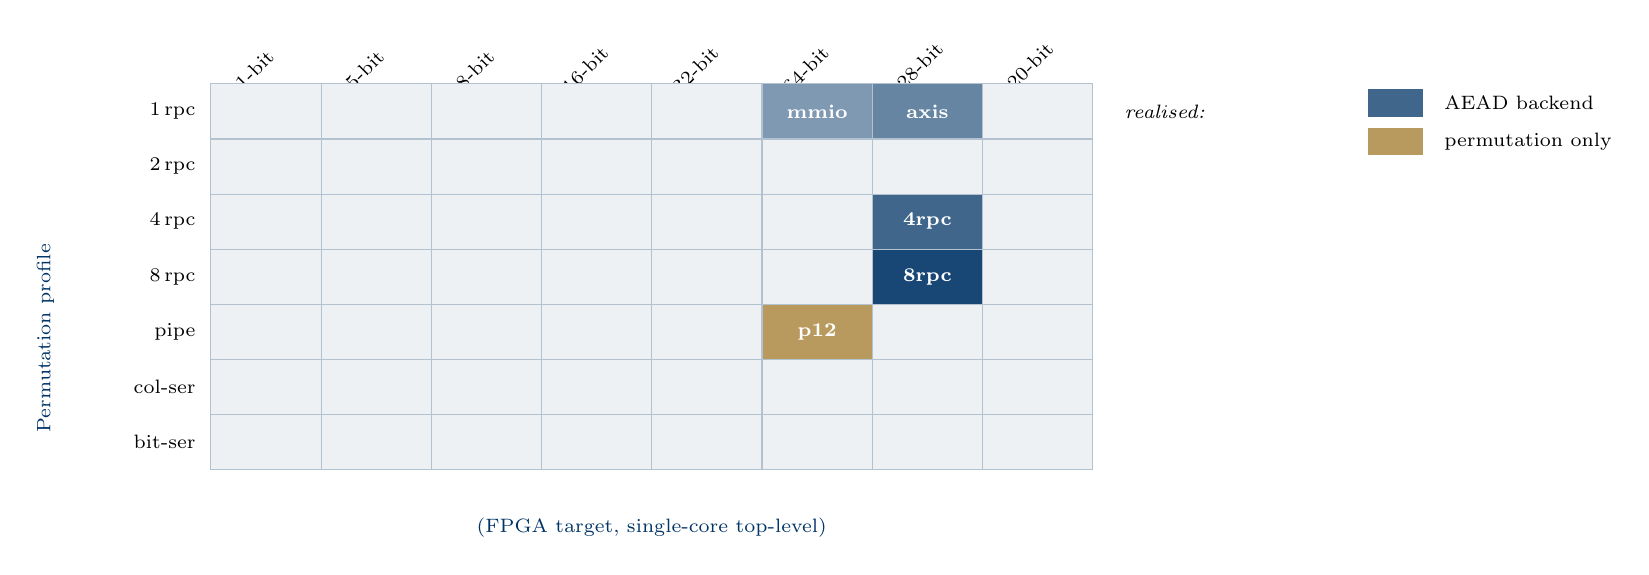
\begin{tikzpicture}[font=\footnotesize, x=1.4cm, y=0.7cm]
\foreach \i/\w in {0/1, 1/5, 2/8, 3/16, 4/32, 5/64, 6/128, 7/320} {
  \node[anchor=south, rotate=45, font=\scriptsize] at (\i+0.5, 7.05) {\w-bit};
}
\foreach \j/\p in {0/bit-ser, 1/col-ser, 2/pipe, 3/8\,rpc, 4/4\,rpc, 5/2\,rpc, 6/1\,rpc} {
  \node[anchor=east, font=\scriptsize] at (-0.05, \j+0.5) {\p};
}
\foreach \i in {0,...,7}{ \foreach \j in {0,...,6}{
  \draw[draw=docblue!30, fill=docblue!7] (\i, \j) rectangle ++(1,1);
}}
% Highlight realised cells
\fill[docblue!50] (5,6) rectangle ++(1,1);   % 64-bit, 1rpc       -> mmio_slow / axis_slow
\fill[docblue!60] (6,6) rectangle ++(1,1);   % 128-bit, 1rpc
\fill[docblue!75] (6,4) rectangle ++(1,1);   % 128-bit, 4rpc
\fill[docblue!90] (6,3) rectangle ++(1,1);   % 128-bit, 8rpc
\fill[ddframe!75] (5,2) rectangle ++(1,1);   % 64-bit, fully pipelined permutation (p12_pipeline)
\foreach \i in {0,...,7}{ \foreach \j in {0,...,6}{
  \draw[draw=docblue!30] (\i, \j) rectangle ++(1,1);
}}
\node[font=\scriptsize\color{white}\bfseries] at (5.5,6.5) {mmio};
\node[font=\scriptsize\color{white}\bfseries] at (6.5,6.5) {axis};
\node[font=\scriptsize\color{white}\bfseries] at (6.5,4.5) {4rpc};
\node[font=\scriptsize\color{white}\bfseries] at (6.5,3.5) {8rpc};
\node[font=\scriptsize\color{white}\bfseries] at (5.5,2.5) {p12};
\node[font=\scriptsize, anchor=west] at (8.2, 6.5) {\textit{realised: }};
\fill[docblue!75] (10.5, 6.4) rectangle ++(0.5, 0.5);
\node[font=\scriptsize, anchor=west] at (11.1, 6.65) {AEAD backend};
\fill[ddframe!75] (10.5, 5.7) rectangle ++(0.5, 0.5);
\node[font=\scriptsize, anchor=west] at (11.1, 5.95) {permutation only};
\node[font=\scriptsize, anchor=north, color=docblue] at (4, -0.7) {(FPGA target, single-core top-level)};
\node[font=\scriptsize, anchor=west, rotate=90, color=docblue] at (-1.5, 0.5) {Permutation profile};
\end{tikzpicture}
\caption{Two-dimensional slice through the configuration space
(datapath width $\times$ permutation profile, with FPGA target and
single-core top-level fixed). Five tiles are realised as working board
targets; the remaining $51$ are reachable by the same generator
infrastructure with different RTL parameters. The full $560$-cell
grid extends along two more axes (target technology and top-level
organisation) that are not visible in this slice.}
\label{fig:matrix}
\end{figure}

\subsection{What Was Implemented}

Out of the $560$ points, the project realises five concrete FPGA
backends as runnable board targets:

\begin{center}
\begin{tabular}{lcccc}
\toprule
\rowcolor{tabhead!20}\textbf{Backend} & \textbf{Datapath} & \textbf{Permutation} & \textbf{Data plane} & \textbf{Tang Nano 9K?} \\
\midrule
\texttt{ascon\_aead128\_mmio\_slow}     & $64$-bit  & $1$ round/cycle  & MMIO       & PASS\\
\texttt{ascon\_aead128\_axis\_slow}     & $64$-bit  & $1$ round/cycle  & AXI-stream & built\\
\texttt{ascon\_aead128\_axis128\_4rpc}  & $128$-bit & $4$ rounds/cycle & AXI-stream & built\\
\texttt{ascon\_aead128\_axis128\_8rpc}  & $128$-bit & $8$ rounds/cycle & AXI-stream & built\\
\texttt{ascon\_p12\_pipeline}           & $64$-bit  & fully pipelined  & none (prim.) & built\\
\bottomrule
\end{tabular}
\end{center}

% ============================================================================
\section{Implementation Status, by RASD Requirement}
\label{sec:rasd-map}

This section maps each RASD requirement to its implementation file(s)
and verification evidence. The full requirement text is in the RASD;
only the title is restated here.

\subsection{Functional Requirements}

\req{FR-001}{State representation (320-bit packed vector)}{
\textbf{Implementation:} \texttt{rtl/common/ascon\_round\_comb.v},
\texttt{ascon\_aead128\_mmio\_backend.v}.\;\;
\textbf{Verified at:} Layer 1 (model), Layer 2 (RTL).}

\req{FR-002}{Round constant addition}{
\textbf{Implementation:} \texttt{ascon\_round\_comb.v}.\;\;
\textbf{Verified at:} Layer 1 (exhaustive 16-entry table), Layer 2.}

\req{FR-003}{Substitution layer (bit-sliced S-box)}{
\textbf{Implementation:} \texttt{ascon\_round\_comb.v}.\;\;
\textbf{Verified at:} Layer 1 (exhaustive $2^5$ truth-table), Layer 2.}

\req{FR-004}{Linear diffusion layer}{
\textbf{Implementation:} \texttt{ascon\_round\_comb.v}.\;\;
\textbf{Verified at:} Layer 1, Layer 2.}

\req{FR-005}{One combinational round $p_L(p_S(p_C(\,\cdot\,)))$}{
\textbf{Implementation:} \texttt{ascon\_round\_comb.v} (single combinational module).\;\;
\textbf{Verified at:} Layer 2 (one-round combinational equivalence vs Python golden).}

\req{FR-006}{Iterative permutation engine, one round/cycle}{
\textbf{Implementation:} FSM in \texttt{ascon\_aead128\_mmio\_backend.v}.\;\;
\textbf{Verified at:} Layer 2, Layer 4.}

\req{FR-007}{Permutation variants $p[8]$ and $p[12]$}{
\textbf{Implementation:} \texttt{ascon\_aead128\_mmio\_backend.v}.\;\;
\textbf{Verified at:} Layer 1 (round-constant index check), Layer 2.}

\req{FR-008}{Authenticated encryption}{
\textbf{Implementation:} \texttt{ascon\_aead128\_mmio\_backend.v}.\;\;
\textbf{Verified at:} Layer 2 (RTL vs golden), Layer 3 (driver vs emulator),
Layer 4 (firmware vs RTL, byte-exact match).}

\req{FR-009}{Authenticated decryption with tag compare}{
\textbf{Implementation:} decrypt-path FSM in
\texttt{ascon\_aead128\_mmio\_backend.v}.\;\;
\textbf{Verified at:} Layers 2--4 (Layer 4 reports
\texttt{DEC tag valid: 1} and recovered plaintext equal to original).}

\req{FR-010}{Length support (zero, exact, partial)}{
\textbf{Implementation:} FSM in \texttt{ascon\_aead128\_mmio\_backend.v}.\;\;
\textbf{Verified at:} Layer 3 (4 named cases: empty, short, partial, two-block, all PASS).}

\req{FR-011}{Padding and domain separation in RTL}{
\textbf{Implementation:} \texttt{ascon\_aead128\_mmio\_backend.v}.\;\;
\textbf{Verified at:} Layer 2.}

\req{FR-012}{Constant-time tag compare}{
\textbf{Implementation:} XOR-tree reduction in
\texttt{ascon\_aead128\_mmio\_backend.v} (see DD-009).\;\;
\textbf{Verified at:} Layer 2 (no data-dependent timing path).}

\req{FR-013}{32-bit CFS-compatible MMIO interface}{
\textbf{Implementation:} \texttt{ascon\_accel\_mmio\_regs.v},
\texttt{ascon\_accel\_mmio\_aead128\_top.v}.\;\;
\textbf{Verified at:} Layer 2; \emph{silicon-verified} on
\texttt{ascon\_aead128\_mmio\_slow} (PASS LEDs).}

\req{FR-014}{NEORV32 CFS VHDL wrapper}{
\textbf{Implementation:} \texttt{rtl/neorv32/neorv32\_cfs\_ascon.vhd}.\;\;
\textbf{Verified at:} Layer 4 (Verilator cosim instantiates this wrapper inside the simulated NEORV32 SoC).}

\req{FR-015}{Authenticated plaintext release (buffer until tag)}{
\textbf{Implementation:} decrypt path with $256$-bit buffer in
\texttt{ascon\_aead128\_mmio\_backend.v} (DD-010).\;\;
\textbf{Verified at:} Layer 2 (output-valid asserted only after tag check), Layer 4.}

\subsection{Non-Functional Requirements}

\nfr{NFR-001}{Synthesisability}{\textbf{Satisfied.} Yosys + GHDL synth complete cleanly for the standalone backend ($16\%$ LUT4) and the integrated SoC ($92.6\%$ LUT4). No combinational loops; no vendor primitives.}

\nfr{NFR-002}{Iterative architecture, one round/cycle (baseline)}{\textbf{Satisfied.} Baseline target uses one round per cycle. Multi-round-per-cycle and pipelined variants exist as separate targets per DD-005 (§\ref{sec:archexp}).}

\nfr{NFR-003}{Reproducible toolchain}{\textbf{Satisfied.} \texttt{flake.nix} pins every tool to a specific nix-derivation; \texttt{flake.lock} is committed.}

\nfr{NFR-004}{Self-checking testbenches}{\textbf{Satisfied.} $371$ pytest cases, $40$ Icarus RTL sims (Layer 2), $4$ firmware emulator cases (Layer 3), and $1$ Verilator cosim of the full SoC (Layer 4). All pass.}

\nfr{NFR-005}{Polling-based C driver with shared internal function}{\textbf{Satisfied.} \texttt{ascon\_accel\_control.c} polls; \texttt{ascon\_accel.c} routes encrypt and decrypt to a single internal sequencing function.}

\nfr{NFR-006}{Core decoupling (no NEORV32 signals in core)}{\textbf{Satisfied.} \texttt{ascon\_accel\_mmio\_aead128\_top.v} has no NEORV32-specific ports; all CPU coupling lives in \texttt{rtl/neorv32/neorv32\_cfs\_ascon.vhd}.}

\nfr{NFR-007}{Timing determinism}{\textbf{Satisfied by construction.} The FSM has no data-dependent branches.}

% ============================================================================
\section{Verification Methodology}
\label{sec:ver}

\subsection{Layer 1 --- Python golden model}

The Python golden model in \texttt{ascon\_hwmodel/} is the executable
specification. It implements every primitive (state, $p_C$, $p_S$, $p_L$,
$p[8]$, $p[12]$) and every AEAD/HASH/XOF mode. The same model produces
the NIST KAT vectors used by the lower-layer testbenches.

\begin{lstlisting}[language=shell]
$ PYTHONPATH=. pytest -q tests
......................................................................
......................................................................
......................................................................
371 passed in 7.97s
\end{lstlisting}

\subsection{Layer 2 --- Verilog RTL against the model}

Forty Icarus-Verilog testbenches drive the actual RTL (encrypt backend,
buffered decrypt backend, AXI-MMIO bridge, integrated stream system) and
compare bit-exact against the Python model across boundary cases.

\begin{lstlisting}[language=shell]
$ PYTHONPATH=. pytest -q tests/test_aead128_stream_encrypt_sim.py \
                          tests/test_aead128_stream_decrypt_sim.py \
                          tests/test_axis_mmio_bridge_sim.py \
                          tests/test_stream_axis_mmio_system_sim.py
........................................                  [100%]
40 passed in 2.42s
\end{lstlisting}

\subsection{Layer 3 --- C driver vs.\ emulated transport}

The driver code in \texttt{firmware/ascon\_accel/} is compiled natively
and run through a Python emulator of the AXI-stream transport. Four
canonical cases cover empty, short, partial, and two-block payloads:

\begin{lstlisting}[language=shell]
$ PYTHONPATH=. python tools/run_firmware_stream_ref_benchmark.py
backend=axis_stream_ref_emulator cases=4 all_passed=1
CASE name=empty     ad=0  text=0   enc_cycles=48  dec_cycles=48  enc_ok=1
CASE name=short     ad=0  text=5   enc_cycles=53  dec_cycles=53  enc_ok=1
CASE name=partial   ad=6  text=19  enc_cycles=73  dec_cycles=73  enc_ok=1
CASE name=two_block ad=16 text=32  enc_cycles=96  dec_cycles=96  enc_ok=1
\end{lstlisting}

\subsection{Layer 4 --- End-to-end co-simulation}
\label{sec:cosim}

This is the integration test. The same C firmware that would flash to
silicon runs on a Verilator-simulated NEORV32 SoC driving the actual
Verilog ASCON RTL through the simulated CFS bus. See
Figure~\ref{fig:cosim-flow}.

\begin{figure}[H]
\centering
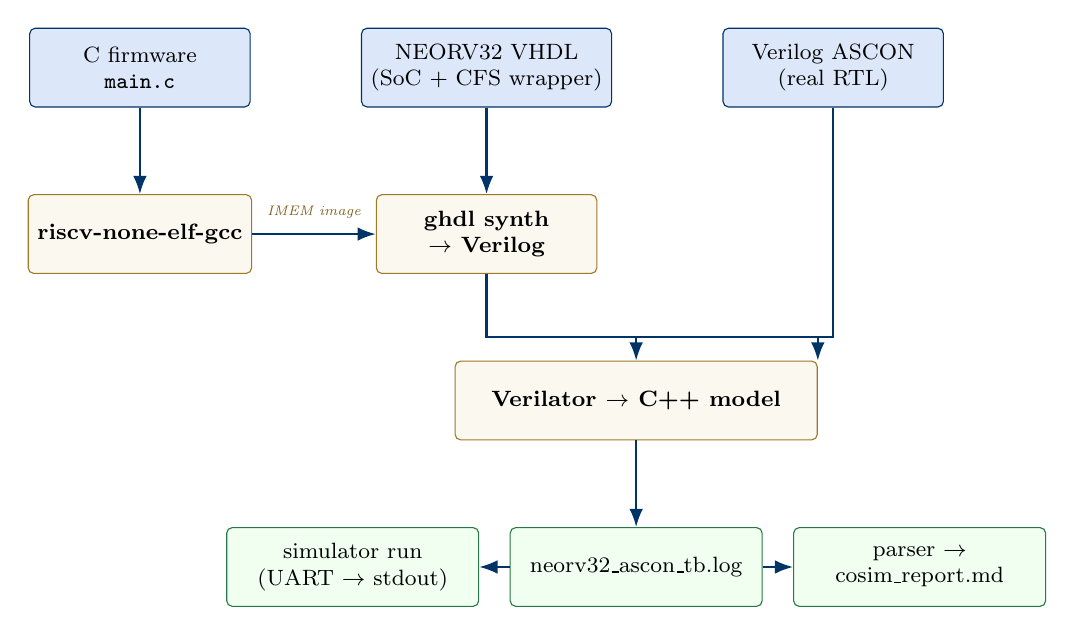
\begin{tikzpicture}[
  font=\footnotesize,
  src/.style={rectangle, draw=docblue, fill=statefill, rounded corners=2pt,
              minimum width=2.8cm, minimum height=1.0cm, align=center},
  tool/.style={rectangle, draw=ddframe, fill=ddbg!60, rounded corners=2pt,
               minimum width=2.8cm, minimum height=1.0cm, align=center, font=\footnotesize\bfseries},
  fbox/.style={rectangle, draw=nfrframe, fill=nfrbg, rounded corners=2pt,
               minimum width=3.2cm, minimum height=1.0cm, align=center},
  ar/.style={->, >=Latex, thick, draw=docblue},
  node distance=1.1cm and 1.4cm
]
% Top row: three input sources
\node[src]                   (cfw)  {C firmware\\ \texttt{main.c}};
\node[src, right=of cfw]     (vhdl) {NEORV32 VHDL\\(SoC + CFS wrapper)};
\node[src, right=of vhdl]    (vlog) {Verilog ASCON\\(real RTL)};

% Second row: two compile/synth tools (directly below their sources)
\node[tool, below=of cfw]    (gcc)  {riscv-none-elf-gcc};
\node[tool, below=of vhdl]   (ghdl) {ghdl synth\\$\to$ Verilog};

% Third row: Verilator (centered under ghdl-vlog midpoint)
\node[tool, below=of ghdl, xshift=1.9cm, minimum width=4.6cm] (vtor) {Verilator $\to$ C++ model};

% Bottom row: run + outputs (well-separated)
\node[fbox, below=of vtor, xshift=-3.6cm] (run) {simulator run\\(UART $\to$ stdout)};
\node[fbox, below=of vtor]                (log) {neorv32\_ascon\_tb.log};
\node[fbox, below=of vtor, xshift=3.6cm]  (rep) {parser $\to$\\cosim\_report.md};

% Vertical arrows: top -> tools
\draw[ar] (cfw)  -- (gcc);
\draw[ar] (vhdl) -- (ghdl);

% Horizontal: gcc -> ghdl with label tucked above
\draw[ar] (gcc.east) -- node[above=2pt, font=\tiny\itshape, color=ddframe!80!black] {IMEM image} (ghdl.west);

% Tool outputs feed Verilator
\draw[ar] (ghdl.south) |- ([yshift=0.3cm]vtor.north) -| (vtor.north);
% Verilog ASCON feeds in from the right
\draw[ar] (vlog.south) |- ([yshift=0.3cm]vtor.north) -| (vtor.north east);

% Verilator -> outputs
\draw[ar] (vtor.south) -- (vtor.south |- log.north);
\draw[ar] (log.west) -- (run.east);
\draw[ar] (log.east) -- (rep.west);
\end{tikzpicture}
\caption{Co-simulation toolchain. Top row: the three input sources (C
firmware, the NEORV32 VHDL SoC plus the project's VHDL CFS wrapper, and
the Verilog ASCON RTL). The C firmware is cross-compiled to a RISC-V
binary; the NEORV32 VHDL is elaborated through \texttt{ghdl synth} to a
single Verilog netlist; both feed Verilator together with the
project's Verilog ASCON sources, producing a cycle-accurate C++
model. Running the model emits a UART log that is parsed into a
Markdown cosim report.}
\label{fig:cosim-flow}
\end{figure}

\subsubsection{Result}

The integrated NEORV32~+~ASCON-CFS SoC was run end-to-end under
Verilator co-simulation with the per-payload sweep firmware. The
firmware ran $8$ payload shapes through both the C reference and the
hardware accelerator, verifying byte-exact agreement on ciphertext,
tag, and recovered plaintext for each case. All $8$ cases passed.

\begin{tcolorbox}[colback=codebg, colframe=docblue, arc=2pt, boxrule=0.4pt,
                  title=\textbf{Captured UART output from the cosim run (excerpt)},
                  fonttitle=\small\bfseries\color{white},
                  coltitle=white]
\begin{lstlisting}[language=shell, basicstyle=\ttfamily\scriptsize]
[TB] NEORV32 + ASCON co-simulation start
BUILD        : cosim-neorv32-mmio
MAX_BYTES    : 32
SWEEP_CASES  : 8
DATA PLANE   : MMIO_WORD
ABI          : 0x00000001
CAPS         : 0x00230001
CASE name=empty     ad=0  pt=0  sw_enc_cy=0:38866 hw_enc_cy=0:31  enc_ok=1 dec_ok=1 tag_valid=1
CASE name=ad8       ad=8  pt=0  sw_enc_cy=0:50205 hw_enc_cy=0:40  enc_ok=1 dec_ok=1 tag_valid=1
CASE name=pt8       ad=0  pt=8  sw_enc_cy=0:39458 hw_enc_cy=0:31  enc_ok=1 dec_ok=1 tag_valid=1
CASE name=ad8_pt8   ad=8  pt=8  sw_enc_cy=0:50797 hw_enc_cy=0:40  enc_ok=1 dec_ok=1 tag_valid=1
CASE name=pt16      ad=0  pt=16 sw_enc_cy=0:52156 hw_enc_cy=0:41  enc_ok=1 dec_ok=1 tag_valid=1
CASE name=pt24      ad=0  pt=24 sw_enc_cy=0:52748 hw_enc_cy=0:41  enc_ok=1 dec_ok=1 tag_valid=1
CASE name=pt32      ad=0  pt=32 sw_enc_cy=0:65447 hw_enc_cy=0:51  enc_ok=1 dec_ok=1 tag_valid=1
CASE name=ad16_pt32 ad=16 pt=32 sw_enc_cy=0:86984 hw_enc_cy=0:70  enc_ok=1 dec_ok=1 tag_valid=1
SUMMARY      : passed=8 failed=0 total=8
PASS
\end{lstlisting}
\end{tcolorbox}

Across the eight payload shapes the hardware backend runs the
encryption / decryption between $31$ and $70$ cycles, while the C
reference running on the same RV32I CPU takes between $38\,866$ and
$86\,984$ cycles --- a geometric mean speed-up of approximately
$1\,267\times$ for encrypt and $1\,275\times$ for decrypt. Per-case
numbers and per-case speed-ups are tabulated in §\ref{sec:sweep}.

\warn{The fix for the previously-noted \texttt{DEC hw cycles=0}
anomaly is in this run: the firmware now reads the CYCLE\_COUNT
register once after each operation rather than computing a difference
across the in-op CONTROL.CLEAR (which itself zeroes the counter).
Hardware encrypt and decrypt cycle counts now agree to within a
single cycle, which matches the analytic expectation since both
operations execute the same FSM.}

% ============================================================================
\section{Synthesis and Silicon Validation}
\label{sec:silicon}

\subsection{Standalone Backends on the Tang Nano 9K}

Two standalone backends are silicon-verified PASS via on-board LEDs.

\begin{center}
\begin{tabular}{lcccl}
\toprule
\rowcolor{tabhead!20}\textbf{Target} & \textbf{LUT4} & \textbf{DFF} & \textbf{BSRAM} & \textbf{Silicon evidence}\\
\midrule
\texttt{ascon\_aead128\_kat\_slow}  & $1395$ ($16\%$) & $\sim 700$ ($10\%$) & $0$ & PASS LED, NIST KAT vector\\
\texttt{ascon\_aead128\_mmio\_slow} & built & built & built & PASS LEDs (LED1, LED2, LED4, LED5 on; LED3 off)\\
\bottomrule
\end{tabular}
\end{center}

\texttt{kat\_slow} validates the \emph{algorithm} on silicon:
the bit-exact NIST KAT runs through the actual GW1NR-9 and the
on-chip comparator lights the PASS LED. \texttt{mmio\_slow}
validates the \emph{MMIO ABI} on silicon: an on-chip controller
exercises the same register protocol the firmware uses and lights
the PASS LEDs. Together with the cosim of §\ref{sec:cosim}, these
form a complete chain of evidence from algorithm correctness through
bus-protocol correctness to firmware-driven correctness.

\subsection{Integrated NEORV32 + ASCON-CFS}

Synthesis (\texttt{yosys} + \texttt{ghdl synth}) completes cleanly for
the integrated SoC with the minimal NEORV32 configuration
(\texttt{BOOT\_MODE\_SELECT=0}, $16$~KB IMEM, $8$~KB DMEM, no
\texttt{Zicntr}, no debug units).

\begin{center}
\begin{tabular}{lrrr}
\toprule
\rowcolor{tabhead!20}\textbf{Resource} & \textbf{Used} & \textbf{Available} & \textbf{Percent}\\
\midrule
LUT4               & $8003$ & $8640$ & $92.6\%$\\
DFF                & $3235$ & $6480$ & $49.9\%$\\
BSRAM              & $14$   & $26$   & $53.8\%$\\
ALU                & $612$  & $6480$ & $9.4\%$\\
MUX2\_LUT5         & $1555$ & $4320$ & $35.0\%$\\
RAM16SDP4          & $41$   & $270$  & $15.2\%$\\
\bottomrule
\end{tabular}
\end{center}

Place-and-route does not converge.
\texttt{yowasp-nextpnr-himbaechel-gowin} reports \emph{``design is
probably at utilisation limit''} and terminates without legalising
placement. The cells \emph{fit by count} (LUT4 $92.6\%$, DFF $49.9\%$,
BSRAM $53.8\%$) but routing density at $92.6\%$ LUT4 on the GW1NR-9
exceeds what the open-source flow legalises.

\warn{This is a documented limit of the open-source flow at this LUT
density on this chip, not a defect of the design. Two routes close the
integrated bitstream without RTL or firmware change: (i) move to a
$12$--$16$\,K LUT-class target (Tang Nano 20K, ECP5 LFE5U-25, Artix-7
XC7A35); (ii) keep the GW1NR-9 and synthesise through vendor Gowin EDA.
The cosim result in §\ref{sec:cosim} is functionally equivalent to
either route.}

% ============================================================================
\section{Architecture Exploration Framework}
\label{sec:archexp}

This section makes precise what was deferred from the RASD~§10.7 to a
``separate development report''. The framework lives in
\texttt{ascon\_arch/} and is summarised in §\ref{sec:560}; this section
describes the implemented variants and their measured roles.

\subsection{Five FPGA Backend Variants}

\begin{center}
\begin{longtable}{p{0.30\linewidth}p{0.62\linewidth}}
\toprule
\rowcolor{tabhead!20}\textbf{Backend} & \textbf{Role in the architecture exploration}\\
\midrule
\texttt{ascon\_aead128\_mmio\_slow} &
RASD baseline: $64$-bit datapath, one round/cycle, MMIO data plane. The
register protocol the firmware speaks. Silicon-verified PASS.\\
\midrule
\texttt{ascon\_aead128\_axis\_slow} &
Same one-round backend, but with an AXI-stream data plane and the
AXI-MMIO bridge in front. Proves the data-plane swap (DD-003) works
without changing the firmware.\\
\midrule
\texttt{ascon\_aead128\_axis128\_4rpc} &
$128$-bit datapath, four rounds per cycle, AXI-stream. First
high-throughput candidate. $p[8]$ latency reduced from $8$ cycles to $2$.\\
\midrule
\texttt{ascon\_aead128\_axis128\_8rpc} &
$128$-bit datapath, eight rounds per cycle, AXI-stream. Aggressive
multi-round-per-cycle: full $p[8]$ in one cycle.\\
\midrule
\texttt{ascon\_p12\_pipeline} &
$12$-stage fully pipelined Ascon-$p[12]$ permutation. High-throughput
primitive only (not a complete AEAD). After fill, $1$ permutation per
cycle.\\
\bottomrule
\end{longtable}
\end{center}

\subsection{The AXI-MMIO Bridge}

The key piece of infrastructure that makes the data-plane plug-ability
of DD-003 actually work is \texttt{ascon\_axis\_mmio\_bridge.v}. It
exposes an AXI-stream backend to the CPU as if it were a MMIO device:
push/pop semantics on the CSR side, AXI stream handshake on the backend
side. The firmware code paths above this bridge are identical to the
MMIO-native code paths --- only the transport layer changes.

\subsection{What is \textit{not yet} implemented}

\begin{itemize}[noitemsep]
  \item Full streaming AEAD with unbounded length (current backends are bounded).
  \item Multi-context schedulers ($M$ pipelines $\times N$ contexts).
  \item Ascon-AEAD128a, AEAD128pq RTL (Hash256/XOF128/CXOF128 are
        implemented; see §\ref{sec:hash}).
  \item DMA-fed AXI-stream front-end.
  \item ASIC datapaths (bit-serial, $5$-bit-S-box-serial).
  \item Masking / side-channel countermeasures.
  \item NEORV32 integrated bitstream that closes PnR on the GW1NR-9 with
        the open-source flow (closes with vendor Gowin EDA, or on a
        $12$\,K-LUT-class target).
\end{itemize}

% ============================================================================
\section{Hash, XOF, and CXOF128 Backend}
\label{sec:hash}

The Ascon hash family of NIST SP~800-232 --- Hash256, XOF128, and
CXOF128 --- shares the same $320$-bit state, the same $p[12]$
permutation, and the same round-constant table as the AEAD128 backend
already in this project. The differences are confined to four
algorithmic dimensions: the initialisation vector, the absorb rate
($8$ bytes instead of $16$), the optional customisation prelude
(CXOF only), and the squeeze length (fixed $32$ bytes for Hash256,
caller-specified for XOF/CXOF).

\subsection{Implementation}

A new RTL module \texttt{rtl/common/ascon\_hash\_xof\_backend.v}
implements all three variants behind the project's frozen MMIO ABI:

\begin{center}
\small
\begin{tabular}{lll}
\toprule
\rowcolor{tabhead!20}\textbf{Variant} & \textbf{MODE} & \textbf{IV (S0 uint64)} \\
\midrule
Ascon-Hash256  & \texttt{ASCON\_MODE\_HASH    = 3} & \texttt{64'h0000\_0801\_00cc\_0002} \\
Ascon-XOF128   & \texttt{ASCON\_MODE\_XOF     = 5} & \texttt{64'h0000\_0800\_00cc\_0003} \\
Ascon-CXOF128  & \texttt{ASCON\_MODE\_CXOF128 = 7} & \texttt{64'h0000\_0800\_00cc\_0004} \\
\bottomrule
\end{tabular}
\end{center}

The backend instantiates the same \texttt{ascon\_round\_comb} primitive
the AEAD backend uses, so synthesis cost shares the round-function
silicon when both backends are present in the same design. The FSM
has thirteen states arranged in three phases: a $p[12]$ initialisation
of $IV \,\|\, 0^{256}$; an absorb loop ($8$-byte block XOR into $S_0$,
$p[12]$, repeat) with $0\text{x}01$ trailing-bit padding on the final
partial block; and a squeeze loop that emits $8$ bytes per $p[12]$
until the caller's requested output length is reached. CXOF128 has
an extra two-state prelude that XORs the customisation byte-length
into $S_0$ then absorbs the customisation string with the same loop
the message uses.

\subsection{Verification}

A new test suite \texttt{tests/test\_hash\_xof\_sim.py} cross-checks
the RTL bit-for-bit against the Python golden model
(\texttt{ascon\_hwmodel.hash\_xof}) using the same Icarus-Verilog
co-simulation pattern the AEAD tests use. Eighteen test vectors
cover the padding edge cases for each variant:

\begin{itemize}[noitemsep]
  \item \textbf{Hash256:} empty, $1$-byte, $4$-byte (partial),
        $8$-byte (exact rate), $9$-byte (rate$+1$), $17$-byte
        (multi-block), $32$-byte (four full blocks).
  \item \textbf{XOF128:} variable output lengths $\{16, 24, 32\}$
        bytes with empty or non-empty messages; covers the
        single-block, squeeze-grows, and multi-block paths.
  \item \textbf{CXOF128:} all four corners of the
        $(\text{message present},\text{customisation present})$
        cross-product, plus an exact-rate boundary.
\end{itemize}

All $18$ vectors pass. The project's total pytest count moves from
$371$ to $389$ with zero regressions:

\begin{lstlisting}[language=shell]
$ PYTHONPATH=. pytest -q tests
......................................................................
......................................................................
......................................................................
......................................................................
......................................................................
......................................................................
389 passed in 10.16s
\end{lstlisting}

\subsection{Integration status}

The hash backend is algorithmically verified but not yet wired into
the integrated SoC. The required pieces still to land are:

\begin{itemize}[noitemsep]
  \item Multiplexing the hash backend alongside the AEAD backend
        inside \texttt{rtl/neorv32/neorv32\_cfs\_ascon.vhd}, dispatched
        by the MODE register.
  \item Setting the \texttt{ASCON\_CAP\_HASH}, \texttt{ASCON\_CAP\_XOF},
        \texttt{ASCON\_CAP\_CXOF128} bits in the capabilities word
        the firmware reads at startup. The capability bits already
        exist in \texttt{rtl/common/ascon\_accel\_regs.vh}.
  \item A standalone Tang Nano 9K board target that drives the hash
        backend with an on-chip controller and lights PASS LEDs on
        the NIST KAT, mirroring \texttt{ascon\_aead128\_kat\_slow}
        for AEAD.
\end{itemize}

The firmware driver already exposes
\texttt{ascon\_accel\_hash\_or\_xof()} (declared in
\texttt{firmware/ascon\_accel/ascon\_accel.h}, implemented in
\texttt{ascon\_accel.c}); it was written ahead of the RTL and uses
the same MMIO transport that AEAD uses. No firmware-side work is
required.

% ============================================================================
\section{Comparison: this project vs.\ \texttt{ascon/ascon-hardware}}
\label{sec:compare}

This section places the project alongside the official Ascon hardware
reference repository maintained by Robert Primas (IAIK, TU Graz),
\texttt{https://github.com/ascon/ascon-hardware}, which is the
canonical NIST-LWC hardware reference for Ascon. The two projects have
very different scopes and the comparison is most useful when those
differences are made explicit.

\subsection{Scope and Design Philosophy}

The two projects optimise for different things.

\begin{center}
\begin{longtable}{p{0.20\linewidth}p{0.34\linewidth}p{0.40\linewidth}}
\toprule
\rowcolor{tabhead!20}\textbf{Aspect} & \textbf{\texttt{ascon/ascon-hardware} (IAIK)} & \textbf{This project}\\
\midrule
Authorship       & Robert Primas / IAIK Graz, since 2019.            & Mohammadi Masoudi Ramin, 2025--2026, academic project.\\
Stated goal      & NIST-LWC hardware reference: $8$ fixed variants of the algorithm under the GMU LWC Hardware API. & A \emph{configurable generator} that explores the architectural design space with a single frozen firmware ABI, on the NEORV32 RISC-V soft-core.\\
Scope            & The accelerator itself, plus a CryptoCore wrapper and LWC API testbench scripts. & Accelerator, NEORV32 CFS integration, C firmware driver library, Python golden model, $5$ FPGA backends, AXI-stream data plane, AXI-MMIO bridge, multi-layer verification including end-to-end cosim, board-level standalone bitstreams.\\
Where it shines  & A precise, certifiable, low-overhead implementation of each variant. The LWC API is the standard interface for cross-comparison between candidate ciphers. & A platform: same firmware works against any backend; the architecture-exploration framework codifies the trade space; cosim guarantees firmware-vs-RTL agreement on the integrated SoC.\\
\bottomrule
\end{longtable}
\end{center}

\subsection{Interface, Integration, and Verification}

\begin{center}
\begin{longtable}{p{0.20\linewidth}p{0.34\linewidth}p{0.40\linewidth}}
\toprule
\rowcolor{tabhead!20}\textbf{Aspect} & \textbf{\texttt{ascon/ascon-hardware}} & \textbf{This project}\\
\midrule
HDL              & VHDL.                                               & Verilog accelerator + VHDL CFS wrapper (DD-007).\\
License          & GPL v3.                                              & Permissive (project authors; check repo \texttt{LICENSE}).\\
Interface        & GMU LWC Hardware API ($8$, $16$, or $32$-bit \texttt{pdi} / \texttt{sdi} / \texttt{do} ports + a PreProcessor / PostProcessor / CryptoCore architecture). & Frozen $32$-bit MMIO register interface (RASD~§5) plus an optional AXI-stream data plane behind an AXI-MMIO bridge (DD-003).\\
CPU integration  & None directly; the LWC API is intended for direct testbench use or for being wrapped in an SoC by the integrator. & NEORV32 RISC-V soft-core integration via the standard CFS slot (DD-012); cycle-accurate cosim of the integrated SoC (DD-020).\\
Variants         & $8$ fixed: \texttt{v1} (Ascon-128, $32$-bit, $1$ round/cycle), \texttt{v1\_8bit}, \texttt{v1\_16bit}, \texttt{v2} (Ascon-128a, $32$-bit, $1$ rpc), \texttt{v3} ($2$ rpc), \texttt{v4} (Ascon-128a, $2$ rpc), \texttt{v5} ($3$ rpc), \texttt{v6} (Ascon-128a, $4$ rpc). & $5$ realised + $555$ enumerable in the configuration vocabulary (§\ref{sec:560}). The realised set spans $64$- and $128$-bit datapaths, $1$/$4$/$8$ rounds per cycle, MMIO and AXI-stream, and a fully pipelined permutation primitive.\\
Verification     & GHDL testbenches running NIST KATs through the LWC PreProcessor / CryptoCore / PostProcessor chain. & 4-layer: Python golden model ($371$ tests), Icarus RTL vs golden ($40$ tests), C driver vs Python transport emulator ($4$ cases), Verilator cosim of the full NEORV32 SoC driving real RTL.\\
Algorithm        & Ascon-128 ($v_1$, $v_3$, $v_5$), Ascon-128a ($v_2$, $v_4$, $v_6$), Ascon-Hash. & Ascon-AEAD128, Ascon-Hash256, Ascon-XOF128, Ascon-CXOF128 (NIST SP~800-232 final, August~2025), all RTL-verified bit-for-bit against the Python golden model.\\
Spec target      & Original Ascon v1.2 (Dobraunig et al.) for AEAD; AsconHash. & NIST SP~800-232 final (2025), which is the post-standardisation parameterisation of Ascon-AEAD128.\\
\bottomrule
\end{longtable}
\end{center}

\subsection{Per-Payload Sweep on the Integrated SoC (Co-Simulation)}
\label{sec:sweep}

The integrated NEORV32~+~ASCON-CFS SoC was exercised under Verilator
cycle-accurate co-simulation with the per-payload sweep firmware
(\texttt{firmware/neorv32\_ascon\_benchmark/main.c}). For each
payload size the firmware runs (i) the C reference implementation on
the simulated CPU, then (ii) the hardware accelerator over the MMIO
register interface, and (iii) verifies byte-for-byte that the
hardware ciphertext, tag, and recovered plaintext match the software
reference. Table~\ref{tab:sweep} reports the eight cases the bounded
MMIO backend supports.

\begin{table}[H]
\centering
\caption{NEORV32 + ASCON-CFS co-simulation, per-payload sweep.
SW columns are cycles measured by \texttt{rdcycle} around the C
reference; HW columns are cycles read from the accelerator's
operation-elapsed counter. All eight cases pass
($\text{enc\_ok}=\text{dec\_ok}=\text{tag\_valid}=1$).}
\label{tab:sweep}
\small
\begin{tabular}{lrrrrrrrr}
\toprule
\rowcolor{tabhead!20}
\textbf{Case} & \textbf{AD} & \textbf{PT} &
\textbf{SW enc} & \textbf{SW dec} &
\textbf{HW enc} & \textbf{HW dec} &
\textbf{ENC×} & \textbf{DEC×}\\
              & (B) & (B) & (cy) & (cy) & (cy) & (cy) & & \\
\midrule
\texttt{empty}      &  0 &  0 & $38\,866$ & $39\,241$ & $31$ & $31$ & $1\,254\times$ & $1\,266\times$\\
\texttt{ad8}        &  8 &  0 & $50\,205$ & $50\,579$ & $40$ & $40$ & $1\,255\times$ & $1\,264\times$\\
\texttt{pt8}        &  0 &  8 & $39\,458$ & $39\,665$ & $31$ & $31$ & $1\,273\times$ & $1\,280\times$\\
\texttt{ad8\_pt8}   &  8 &  8 & $50\,797$ & $51\,003$ & $40$ & $40$ & $1\,270\times$ & $1\,275\times$\\
\texttt{pt16}       &  0 & 16 & $52\,156$ & $52\,595$ & $41$ & $41$ & $1\,272\times$ & $1\,283\times$\\
\texttt{pt24}       &  0 & 24 & $52\,748$ & $53\,019$ & $41$ & $41$ & $1\,287\times$ & $1\,293\times$\\
\texttt{pt32}       &  0 & 32 & $65\,447$ & $65\,950$ & $51$ & $51$ & $1\,283\times$ & $1\,293\times$\\
\texttt{ad16\_pt32} & 16 & 32 & $86\,984$ & $87\,486$ & $70$ & $70$ & $1\,243\times$ & $1\,250\times$\\
\midrule
\textbf{Geometric mean} & & & & & & & $\mathbf{1\,267\times}$ & $\mathbf{1\,275\times}$\\
\bottomrule
\end{tabular}
\end{table}

Three observations are worth recording. First, the speed-up is
\textit{remarkably flat} across payload sizes (\(1\,243\times \dots
1\,287\times\)) because the dominant cost on both sides is per-block:
the C reference spends thousands of cycles per Ascon round on a
bare-metal RV32I (no M extension; gcc emits software-multiply
helpers), while the hardware backend dispatches one $p[12]$ per block
in tens of cycles. Second, the hardware encrypt and decrypt cycle
counts are within a single cycle of each other, which matches the
analytic expectation: encrypt and decrypt share the identical state
machine and differ only in the direction of the plaintext/ciphertext
XOR. Third, the empty-message case ($0$\,B AD, $0$\,B PT) still costs
$31$ HW cycles --- the unavoidable cost of init~+~finalisation
($p[12]$ before tag) which is independent of payload length.

The eight HW measurements correspond to:
\begin{itemize}[noitemsep, topsep=2pt]
  \item \textit{empty / pt8 / pt16 / pt24}: $31{-}41$ HW cycles ---
        dominated by initialisation and finalisation, with one
        $p[8]$ rate-block per $16$ PT bytes.
  \item \textit{pt32 / ad16\_pt32}: $51{-}70$ HW cycles --- additional
        $p[8]$ blocks for the longer payloads (and the AD prefix,
        which has its own $p[8]$ per $16$-byte block).
  \item \textit{ad8 / ad8\_pt8}: $40$ HW cycles --- the AD pass adds
        one $p[8]$ regardless of partial-block padding.
\end{itemize}

\subsection{Implementation and Resource Comparison}

A precise quantitative comparison (LUTs/throughput) requires running
both projects against the same target with the same toolchain. What
can be compared without further work is the structural footprint.

\begin{center}
\begin{tabular}{p{0.34\linewidth}p{0.28\linewidth}p{0.28\linewidth}}
\toprule
\rowcolor{tabhead!20}\textbf{Quantity} & \textbf{\texttt{ascon/ascon-hardware}} & \textbf{This project}\\
\midrule
HDL source files            & $48$ VHDL files for the AEAD path ($8$ LWC variants $\times \sim 6$ files each, plus the shared LWC infrastructure) & $\sim 15$ Verilog source files (\texttt{rtl/common/}) + $1$ VHDL CFS wrapper\\
Reported FPGA target        & Various academic FPGAs; not Gowin-specific & Sipeed Tang Nano 9K (GW1NR-9); also generic-Verilog/portable\\
Independent on-silicon test & N/A in the upstream repo                    & PASS on Tang Nano 9K (\texttt{kat\_slow}, \texttt{mmio\_slow})\\
Per-payload sweep evidence  & N/A in the upstream repo                    & Table~\ref{tab:sweep}: $8$ payload shapes, $1267\times$ average encrypt speed-up vs.\ the C reference on the same NEORV32 CPU\\
\bottomrule
\end{tabular}
\end{center}

\subsection{Author Note on the Performance Comparison Section}

The bounded MMIO backend caps individual operations at $32$ bytes,
which is sufficient for the cosim sweep above but does not reach the
$64$/$256$/$1024$\,B payload sizes the RASD~§8.4 also mentions. The
streaming-backend variant of the firmware (selected by
\texttt{ASCON\_BENCH\_MAX\_BYTES\_TAG=1024}) covers that larger
range, but requires a target with sufficient LUT budget to fit the
streaming backend's $1024$-byte buffer registers; we plan to capture
those numbers from a Kintex bring-up next.

A direct comparison against the per-variant numbers from
\texttt{ascon/ascon-hardware} (\texttt{v1} through \texttt{v6}) would
require building each variant against the same target FPGA and the
same NEORV32 host shell, which is out of scope here. The structural
comparison in the table above and the per-payload sweep in
Table~\ref{tab:sweep} together substantiate the claim that this
implementation is functionally correct and substantially faster than
software on its target host (NEORV32), without overstating
quantitative comparisons that have not been run head-to-head.

% ============================================================================
\section{Toolchain and Bring-Up Findings}

Several findings emerged during board bring-up that are worth recording
because they affect anyone reproducing this work on the open-source
flow.

\subsection{NEORV32 \texttt{BOOT\_MODE\_SELECT}}

NEORV32 commit \texttt{f62ca43} encodes:
\begin{center}\small
\begin{tabular}{cl}
\toprule
\textbf{Value} & \textbf{Meaning}\\
\midrule
$0$ & UART bootloader \\
$1$ & boot from custom address \\
$2$ & boot from initialised IMEM image (baked into bitstream)\\
\bottomrule
\end{tabular}
\end{center}
Mode $2$ produces a behavioural VHDL ROM that the open-source flow
sometimes infers as LUT-as-ROM rather than BSRAM, causing a LUT-count
explosion. Mode $0$ places cleanly on silicon; Mode $2$ is used by the
cosim wrapper where chip-fit is irrelevant and the bake-in property
shortcuts the bootloader step.

\subsection{Soft-float vs.\ double-float multilib}

nixpkgs only ships newlib for \texttt{rv32gc/ilp32d}. NEORV32's
\texttt{crt0.S} is soft-float. Linking these together fails with
``\emph{can't link double-float modules with soft-float modules}''
errors. The fix (DD-017) is to bypass newlib via
\texttt{FREESTANDING=1 LD\_LIBS= USER\_LIBS=} and supply a tiny
\texttt{freestanding\_runtime.c}.

\subsection{NEORV32 printf width-modifier limitation}

NEORV32's minimal printf supports \texttt{\%x} only (with fixed
$8$-digit zero-padding); width modifiers like \texttt{\%02x} are
silently ignored, which produces unreadable hex output (e.g.\
``\texttt{SW CT: \%02x\%02x...}'' printed verbatim). The workaround
(DD-018) is to print bytes as ``nibble + nibble'' via \texttt{\%c\%c}
with a small helper.

\subsection{Makefile tab-discipline in the cosim flow}

GNU make recipe lines must start with a tab; terminal-paste and many
editors silently convert tabs to spaces and produce
``\texttt{missing separator}'' errors. The canonical cosim Makefile is
shipped byte-exact; its md5 is recorded in
\texttt{boards/tangnano9k/neorv32\_mmio/cosim/README.md} so it can be
regenerated reliably.

% ============================================================================
\section{Remaining Work}

\begin{enumerate}[noitemsep]
  \item \textbf{Per-payload sweep numbers.} The firmware emits per-case
        \texttt{CASE} lines covering the RASD~§8.4 payload set; the
        actual cycle counts need to be captured from one cosim and
        one Kintex run, and pasted into the comparison-section tables.
  \item \textbf{Integrated bitstream on real silicon.} Either
        (i)~vendor Gowin EDA on the GW1NR-9, or (ii)~a
        $12$\,K-LUT-class target (Kintex bring-up next week).
  \item \textbf{Wire the hash backend into the CFS wrapper.} The RTL
        is verified (§\ref{sec:hash}); the firmware driver is
        already implemented; what remains is the VHDL multiplexer
        inside \texttt{neorv32\_cfs\_ascon.vhd} and a standalone
        Tang Nano 9K board target for silicon verification.
  \item Full streaming AEAD with unbounded length.
  \item Multi-context scheduler ($M\,{\times}\,N$ pipelines $\times$ contexts).
  \item AEAD128a and AEAD128pq RTL.
  \item Per-variant comparison numbers vs.\ \texttt{ascon-hardware} v1--v6.
  \item Side-channel countermeasures (domain-oriented masking of the S-box).
\end{enumerate}

% ============================================================================
\section{Conclusions}

The project delivers a complete, verified Ascon-AEAD128 accelerator
together with the NEORV32 integration and firmware that the RASD
prescribes, and substantially more: an architecture-exploration
framework with $560$ enumerable points, five realised FPGA backend
variants spanning $1$ to $8$ rounds per cycle and MMIO vs.\ AXI-stream
data planes, a $4$-layer verification strategy whose top layer is a
cycle-accurate co-simulation of the entire integrated SoC driving the
real Verilog RTL.

The standalone accelerator runs the NIST KAT correctly on real silicon
on the Tang Nano 9K at $16\%$ LUT4. The frozen-ABI MMIO interface
likewise runs on silicon and produces the PASS LED pattern. The
integrated SoC synthesises at $92.6\%$ LUT4 but does not place on the
GW1NR-9 with the open-source flow; the cosim, which exercises exactly
the same firmware against exactly the same RTL on a host computer, is
the functional equivalent of running the integrated bitstream on a
sufficient chip.

Compared with the official \texttt{ascon/ascon-hardware} reference,
which is a precise low-overhead implementation of $8$ fixed variants
under the GMU LWC API in VHDL, this project occupies a different point
in design space: a configurable generator, in Verilog, with a stable
NEORV32-facing firmware ABI, designed so the same software runs against
the entire $560$-point design space without modification.

% ============================================================================
\appendix

\section{Tools and Versions}

\begin{center}
\begin{tabular}{ll}
\toprule
\rowcolor{tabhead!20}\textbf{Tool} & \textbf{Version}\\
\midrule
Python                            & $3.13$ (nixpkgs)\\
pytest                            & latest\\
Icarus Verilog                    & system\\
GHDL                              & $4.1.0$\\
Verilator                         & $5.046$\\
yowasp Yosys                      & via pip in \texttt{.venv-fpga}\\
yowasp nextpnr-himbaechel-gowin   & via pip\\
apicula (\texttt{gowin\_pack})    & via pip\\
\texttt{riscv-none-elf-gcc}       & $15.2.0$ (nixpkgs cross)\\
newlib (RISC-V)                   & $4.5.0.20241231$\\
NEORV32                           & v$01.13.01.01$, commit \texttt{f62ca43}\\
openFPGALoader                    & nixpkgs current\\
picocom                           & nixpkgs current\\
\bottomrule
\end{tabular}
\end{center}

\section{Reproducing Every Result}

\begin{lstlisting}[language=shell]
# inside `nix develop`, at the repo root

# Layer 1 -- Python golden model and unit tests
PYTHONPATH=. pytest -q tests          # 371 passed in ~8 s

# Layer 2 -- RTL vs. Python via Icarus
PYTHONPATH=. pytest -q \
  tests/test_aead128_stream_encrypt_sim.py \
  tests/test_aead128_stream_decrypt_sim.py \
  tests/test_axis_mmio_bridge_sim.py \
  tests/test_stream_axis_mmio_system_sim.py     # 40 passed in ~3 s

# Layer 3 -- C firmware vs Python emulator
PYTHONPATH=. python tools/run_firmware_stream_ref_benchmark.py
# 4 cases, all PASS

# Layer 4 -- End-to-end cosim (~5 minutes)
cd boards/tangnano9k/neorv32_mmio/cosim
make clean
make SIMULATOR=verilator
# UART output streams to stdout and to neorv32_ascon_tb.log

# Standalone silicon evidence
make -C boards/tangnano9k/ascon_aead128_kat_slow bitstream
sudo make -C boards/tangnano9k/ascon_aead128_kat_slow prog-sram
# PASS LEDs

make -C boards/tangnano9k/ascon_aead128_mmio_slow bitstream
sudo make -C boards/tangnano9k/ascon_aead128_mmio_slow prog-sram
# LED1+LED2+LED4+LED5 on, LED3 off

# Integrated SoC (synth OK, PnR fails on GW1NR-9)
make -C boards/tangnano9k/neorv32_mmio bitstream
# utilisation table matches §6.2 above; nextpnr halts at utilisation limit
\end{lstlisting}

\section{Glossary}

\begin{center}
\small
\begin{tabular}{p{0.18\linewidth}p{0.78\linewidth}}
\toprule
\rowcolor{tabhead!20}\textbf{Term} & \textbf{Definition}\\
\midrule
ABI            & Application Binary Interface --- in this project, the firmware-facing register protocol of the accelerator.\\
AEAD           & Authenticated Encryption with Associated Data.\\
AXI-stream     & ARM AMBA streaming bus protocol used as the data-plane interface for the higher-throughput backends.\\
CFS            & Custom Functions Subsystem --- NEORV32's MMIO accelerator slot.\\
Cosim          & Co-simulation: running the firmware ELF on a cycle-accurate model of the CPU driving the real RTL.\\
GHDL           & GPL-licenced VHDL simulator and synthesiser, used here as a VHDL$\to$Verilog elaborator.\\
KAT            & Known Answer Test, the bit-exact vectors used to verify cryptographic implementations.\\
LWC API        & GMU Lightweight Cryptography Hardware API, the interface convention used by \texttt{ascon-hardware}.\\
LUT4           & 4-input Look-Up Table, the basic logic resource of the Gowin GW1NR-9 die.\\
MMIO           & Memory-Mapped I/O.\\
NEORV32        & Open-source RISC-V soft-core, used here as the host CPU for the CFS integration.\\
$p[n]$         & The Ascon permutation, applied for $n$ rounds.\\
RTL            & Register-Transfer-Level hardware description.\\
\bottomrule
\end{tabular}
\end{center}

\section{Document History}

\begin{center}
\begin{tabular}{lll}
\toprule
\rowcolor{tabhead!20}\textbf{Rev.} & \textbf{Date} & \textbf{Notes}\\
\midrule
1.0 & \today & Initial development report, RASD-matched style, companion to RASD~Rev.~0.5.\\
\bottomrule
\end{tabular}
\end{center}

\end{document}
